\chapter{Implications of codon–anticodon interaction on the regulation of translation}

In the previous chapter I have shown that the codon usage and its interaction
with \trna anticodons remains remarkably stable across the variability of the
transcriptome during mammalian development.

Shortly after the publication of our research on \trna gene regulation during
mouse development, \citet{Gingold:2014} published \texttitle{A Dual Program for
Translation Regulation in Cellular Proliferation and Differentiation}. They
report that different programmes of cellular function preferentially use
different sets of codons, and that the pool of active \trna[s] adapts
dynamically to decode this set of codons with high efficiency.

Because its conclusions are highly relevant to our own research we evaluated the
paper carefully. In the following, I will first describe the paper’s main
findings, to the extent that they are relevant to our own research. I will then
outline our concerns with the analysis, and the subsequent experiments we
performed in an effort to explain how our previous results relate to this paper.

\section{“A dual program for translation regulation in cellular proliferation
and differentiation”}

\citet{Gingold:2014} investigated the abundance of \trna anticodons and the
codon usage of different groups of protein-coding genes in patient tissue
samples and human-derived cell lines in different cellular conditions --- five
primary cancers, induced differentiation, release from serum starvation,
senescence, and \gene{MYC} and \gene{RAS} overexpression --- with the aim of
characterising the differences in \trna gene expression and \trna anticodon
abundance. They hypothesise that the balance between \trna anticodon supply and
codon demand might influence the rate of production of proteins from \mrna
\citep{Gingold:2011}.

\subsection{\abbr{trna} anticodons change in abundance in tumour tissues}

\citet{Gingold:2014} designed custom microarrays for the \trna[s] of most
anticodons present in human, excluding those prone to cross-hybridi\-sation, or
where a low in silico screening score predicts that they may be pseudogenes.
Using these microarrays, they assayed the abundance of anticodon isoacceptors in
healthy B cells and in B-cell derived lymphomas, and show that there are
specific anticodon isoacceptors whose abundance changes reproducibly in tumours
compared to healthy tissue, while other anticodon isoacceptors do not change
their abundance. This mirrors results reported previously
\citep{Pavon-Eternod:2009}.

In addition, they performed the same \trna anticodon abundance analysis on all
samples and applied a hierarchical clustering to the resulting matrix of \trna
expression profiles of all samples. They observe that this clusters samples by
whether they are derived from tumour tissues or from differentiating tissues.
When performing an equivalent clustering on \mrna gene expression values for the
same samples, they observe that samples cluster not by whether they are tumours,
but rather by their tissue of origin, i.e.\ by the tissue from which the tumour
or cell line was derived.

\subsection{Codon usage differs between genes involved in cell proliferation and
genes involved in differentiation}

Next, \citet{Gingold:2014} looked at protein coding genes within \go terms that
they functionally associated with healthy, adult tissue (“pattern specification
process”) on the one hand, and tumour tissue (“M phase of mitotic cell cycle”)
on the other hand. They show that the codon usage bias in these two \go terms
(averaged over all containing genes) clearly differs
(\cref{fig:go-term-codon-usage}): the genes in both \go terms preferentially use
different synonymous codons.\todo{GO annotation for cell cycle etc will contain + and - regulators}

\textfig{go-term-codon-usage}{body}{0.6\textwidth}
    {Codon usage bias in two \abbr{go} terms.}
    {Each point represents one codon, whose corresponding amino acid is given by
    the label. The position of the point is given by the codon usage bias in
    each \go term, respectively. Codons for the same amino acid share the same
    colour (reproduction of figure 2A in \citet{Gingold:2014}).}

They expand their analysis by calculating the mean codon usage across many \go
categories and perform \pca on the resulting matrix (\cref{fig:go-cub-pca}).
This reveals that the largest contributor to the variation stems from the split
of the \go terms into two distinct sets, one encompassing multi-cellular \go
terms and the other cell autonomous \go terms. They argue that these two sets of
\go terms correspond to \go terms functionally responsible for maintaining cell
homoeostasis on the one hand, and rapid cellular division, such as found in
tumours, on the other hand. In other words, different gene families specific to
rapidly dividing as opposed to healthy, mature cells have a distinct codon
composition.\todo{GO hierarchy? Term selection? Slice through GO tree --- remove gene redundancy in sets. Not independent data points}

\textfloat{go-cub-pca}{spill}
    {%
        \begin{minipage}{0.6\textwidth}
            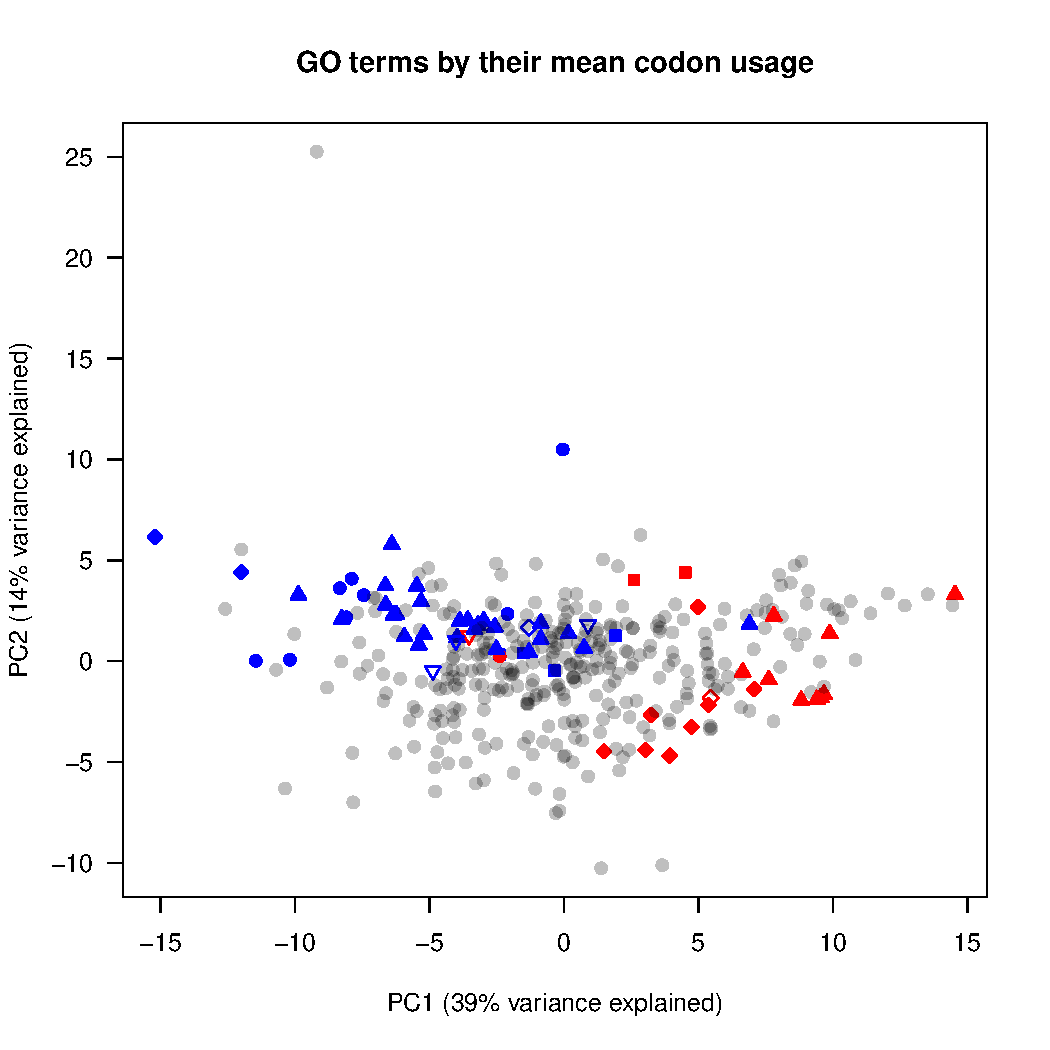
\includegraphics[width=\textwidth]{go-cub-pca}
        \end{minipage}%
        \begin{minipage}{0.4\textwidth}
            \footnotesize\sffamily
            \begin{tabu} to \textwidth {@{}>{\color{blue}\(}c<{\)}X@{}}
                \toprule
                \multicolumn{2}{@{}l}{Multi-cellular} \\
                \quad ▲ & Development \\
                \quad ⬤ & Differentiation \\
                \quad ⬛ & Cell adhesion \\
                \quad ◆ & Pattern specification \\
                \quad ◇ & Multicellular organism growth \\
                \quad ▽ & Angiogenesis \\
                \addlinespace
            \end{tabu}
            \begin{tabu} to \textwidth {@{}>{\color{red}\(}c<{\)}X@{}}
                \multicolumn{2}{@{}l}{Cell autonomous} \\
                \quad ▲ & Mitotic cell cycle \\
                \quad ⬤ & Nucleosome assembly \\
                \quad ⬛ & Chromatin remodelling/modification \\
                \quad ◆ & Translation \\
                \quad ◇ & \mrna metabolic process \\
                \quad ▽ & Negative regulation of cell cycle \\
                \bottomrule
            \end{tabu}
        \end{minipage}
    }
    {\pca of mean \go term codon usage.}
    {Each dot corresponds to one \go term. The position of the dots is derived
    by rotating the matrix of the mean codon usage of the genes belonging to
    each \go term. Created using methods of \citet{Gingold:2014} (the precise
    numbers differ slightly due to the use of different implementations to
    perform the analysis but this does not impact the interpretation).}

\subsection{Differential codon usage in cell-condition specific gene sets
matches \abbr{trna} anticodon abundance in corresponding cells}

Finally, \citet{Gingold:2014} compared the \pca of the per-\go codon usage to
the actual gene expression of \mrna[s] and \trna[s]. The analysis was done in
two parts. Firstly, protein-coding gene expression between normal tissue and
either a tumour sample or a induced differentiation sample was compared, and the
fold change calculated for each gene. The mean fold change of each \go term,
mapped to a colour map, was plotted on top of the \go terms in the \pca
(\cref{fig:gingold-fig-3c} bottom). There seems to be a marked gradient of \mrna
expression enrichment from left to right. This illustrates that the first
principal component of the \pca does indeed separate \go terms by their
specificity to either proliferating or differentiating cellular programmes.

Secondly, to estimate translation efficiency they calculated the change in
abundance of the \trna genes whose isoacceptors decode the codons of the genes
in each \go term, and averaged across them. The fold change in translation
efficiency between healthy tissue and the sample under consideration was again
mapped to a colour gradient, which was overlaid over the \pca
(\cref{fig:gingold-fig-3c} top). Again there appears to be a gradient of how
well different \go terms are adapted to the \trna anticodon pool of a given
condition, following the first principal component of the \pca.

However, the authors did not calculate correlations between the first principal
component and either the codon usage bias or the translation efficiency fold
change. Instead, they merely visualised the presumed correspondence using the
potentially misleading rainbow colour map \citep{Borland:2007}. Furthermore, the
absolute range of changes is minute compared to the overall fold change (range
of fold change \numrange{0.86}{0.905} in one case, corresponding to less than
\num{5} per cent of the maximum fold change), and the lack of statistical
analysis makes it impossible to tell whether these changes are in fact
significant, assuming they correlate at all. It is also worth noting that the
whole fold change range is positive: Even \go categories that are unspecific for
a given condition according to \cref{fig:go-cub-pca} (they fall on the wrong
side of the first principal component), and should thus be less adapted to the
\trna anticodon abundance, are in fact better adapted according to this analysis
(\cref{fig:gingold-fig-3c}). This is a recurring feature for all conditions
tested in this way, and is at odds with the claim that the \trna anticodon pool
is specially adapted to cell condition specific gene sets.

\textfig{gingold-fig-3c}{body}{\textwidth}
    {Projection of the \trna and \mrna expression changes on the codon usage
    map for cells after induced differentiation via retinoic acid.}
    {Both panels show the same \pca as in \cref{fig:go-cub-pca}. In the top
    panel, the colours correspond to the fold change in predicted translation
    efficiency of the genes constituting each \go term, given the change in
    cellular abundance of \trna anticodons compared to normal cells. The bottom
    panel shows the mean fold change in \mrna levels per \go term compared to
    normal cells. Figure from \citet{Gingold:2014}.}

\section{Are \abbr{trna} anticodon abundance and codon usage highly adapted to
different cellular conditions?}

To bring in line these two findings — the stability of the anticodon pool on the
one hand, and the malleability of the anticodon pool to match the codon demand
of highly expressed protein-coding genes on the other hand — we turned our
attention to differences between healthy tissue and tumour cell lines in \mmu
and \hsa.

\subsection{The effect of gene set size on codon usage bias}

Since we were already in possession of relevant \trna data we decided to use our
own data to recapitulate these findings. A first observation was that while our
own research so far had looked at the whole transcriptome, \citet{Gingold:2014}
had looked at specific subsets. While both approaches are valid in their own
right, some caution is necessary when comparing the results: the smaller the set
of genes one looks at, the larger the effects of random sampling of the genes
become. When analysing a particular feature, such as the codon usage bias,
random sampling will thus contribute a larger part to the variation between two
small sets than between two large sets. If one wants to assert that deviations
are nonrandom, one thus has to account for this effect.

To assess how much of the variation in \go term codon usage is explainable by
random variation, I created random sets of different numbers of genes, covering
the whole range of \go term gene set sizes. For each size, I repeatedly sampled
random genes and calculated the mean \rcu of the resulting set. This was done
\num{10000} times for each size. To compare the \rcu variability, each \rcu was
compared to the genome-wide \rcu (i.e.\ using the set of all genes) using
Pearson correlation. \Cref{fig:sample-size-dependent-cub} plots the distribution
of the correlations against the gene set sizes.

\textfig{sample-size-dependent-cub}{spill}{\textwidth}
    {Dependence of codon usage variability on sample size.}
    {Genes were randomly sample from the human genome to create sets of sizes
    given by \(x\) (in grey). The mean codon usage of the sets was calculated,
    and their Pearson correlation to the genomic background is shown on the
    \(y\) axis. Overlaid are actual gene sets given by human \go categories.}

The plot illustrates that few \go categories, if any, can confidently be said to
have a codon usage varying more than just randomly. In addition, the allocation
of individual \go categories to either set can certainly also be criticised: It
is certainly not clear why “translation” should be more active during cellular
division than in stable cells. The authors rather describe the relevant set as
“cell autonomous” \go terms, but the paper’s argument implicitly assumes that
this corresponds to cell division. Furthermore, the allocation of genes to \go
terms was performed via simple textual matching, such that \go sub-categories
whose description contains the text “differentiation and proliferation” would be
counted as belonging to the \go super-category “differentiation”.

\subsection{The extent of anticodon adaptation to distinct cellular conditions}

To test whether the anticodon pool does indeed adapt to specific cellular
conditions as suggested by \cref{fig:gingold-fig-3c}, I examined whether the
codon--anticodon adaptation (estimated via the correlation between matching
codons and anticodons, each as a proportion of the contribution to their
corresponding amino acid, i.e.\ the \rcu and \raa) is higher between matching
\mrna and \trna transcriptomes (measured via \rnaseq and \pol3 \chipseq; using
the same method of quantification as in \cref{seq:trna}) than between
mismatching ones, and whether it is highest in genes that are specific to a
given cellular programme. In other words, I looked at the \mrna pool of each
cellular condition, and calculated the codon--anticodon correlations for

\begin{enumerate}
    \item the whole transcriptome and their matching \trna pool (“matching”),
    \item the whole transcriptome and all mismatching \trna pools
        (“mismatching”),
    \item the differentially, highly expressed \mrna genes and their matching
        \trna pool (“\abbr{de}”), and
    \item condition specific gene sets (for the \go terms “M phase of mitotic
        cell cycle” \& “pattern specification process”) and their matching \trna
        pool (“\abbr{go}”).
\end{enumerate}

The analysis compares different scenarios that should, according to the
hypothesis proposed by \citet{Gingold:2014}, show markedly different
distributions: codon and anticodon pools of the same cellular conditions should
be highly coordinated (correlation type “matching”). Codons and anticodons of
\emph{mismatching} conditions (i.e.\ the codon pool of a healthy cell and the
anticodon pool of a tumour cell, or vice versa) should be less well coordinated
(correlation type “mismatching”). Furthermore, the codon usage of just a subset
of the overall transcriptome corresponding to genes specific to the cellular
condition should be coordinated with their anticodon pool to an even greater
extent. Conversely, if we did not expect a \trna anticodon pool adapted to
specific subsets of the transcriptome, we might expect that the correlation
between the codon usage of such subsets and the anticodon abundance was
\emph{less} than that of the overall transcriptome, due to higher stochastic
variability in smaller gene sets.

Cell specific subsets of the transcriptome can be defined in several ways. My
analysis used two possible definitions: Firstly, I looked at differentially
expressed genes between healthy and tumour cells, and called genes
condition-specific if they were significantly differentially expressed (adjusted
\(p < 0.001\)), their expression was high (mean expression between the
conditions in the upper quartile of all mean expressions), and their fold change
between the conditions was also high (taking the \num{200} genes with the
highest fold change; correlation type “\abbr{de}”). Secondly, I took the gene
sets of the two most extreme \go terms found by \citet{Gingold:2014} according
to the variance in codon usage, which they describe as highly specific for
proliferating cells (\go term “M phase of mitotic cell cycle”) and
differentiating/differentiated cells (\go term “pattern specification process”;
correlation type “\abbr{go}”).

I performed the analysis in \mmu and \hsa. However, \go term annotations vastly
differ between these two species and, in particular, one of the two condition
specific \go terms (according to the \pca analysis, \cref{fig:go-cub-pca}) is
badly annotated in \mmu (with only \num{3} genes annotated for “M phase of
mitotic cell cycle”). As a consequence, I did not use the existing \go term
annotations for mouse but rather used the orthologous gene sets from the human
\go term annotation.

We want to test whether the “mismatching” correlations are lower than the
“matching” ones, but whether the “\abbr{de}” and “\abbr{go}” correlations are
higher, respectively, than the “matching” ones. I therefore used one-tailed
tests for significant difference. In all but one cases, I failed to reject the
null hypothesis of no difference. The only case where we find some support for
rejecting \(H_0\) is the comparison of “matching”--“mismatching” in \hsa (\(p =
0.048\), one-tailed Mann–Whitney–Wilcoxon test). On the other hand, the
“\abbr{go}” correlations are significantly \emph{lower} than the “matching”
correlations in both species (\(p < \num{4.4e-5}\) in \mmu; \(p < \num{2.5e-8}\)
in \hsa). This offers evidence against the hypothesis put forward by
\citet{Gingold:2014} (\cref{fig:cub-aab}).

\textfloat{cub-aab}{spill}
    {%
        \begin{minipage}{0.35\textwidth}
            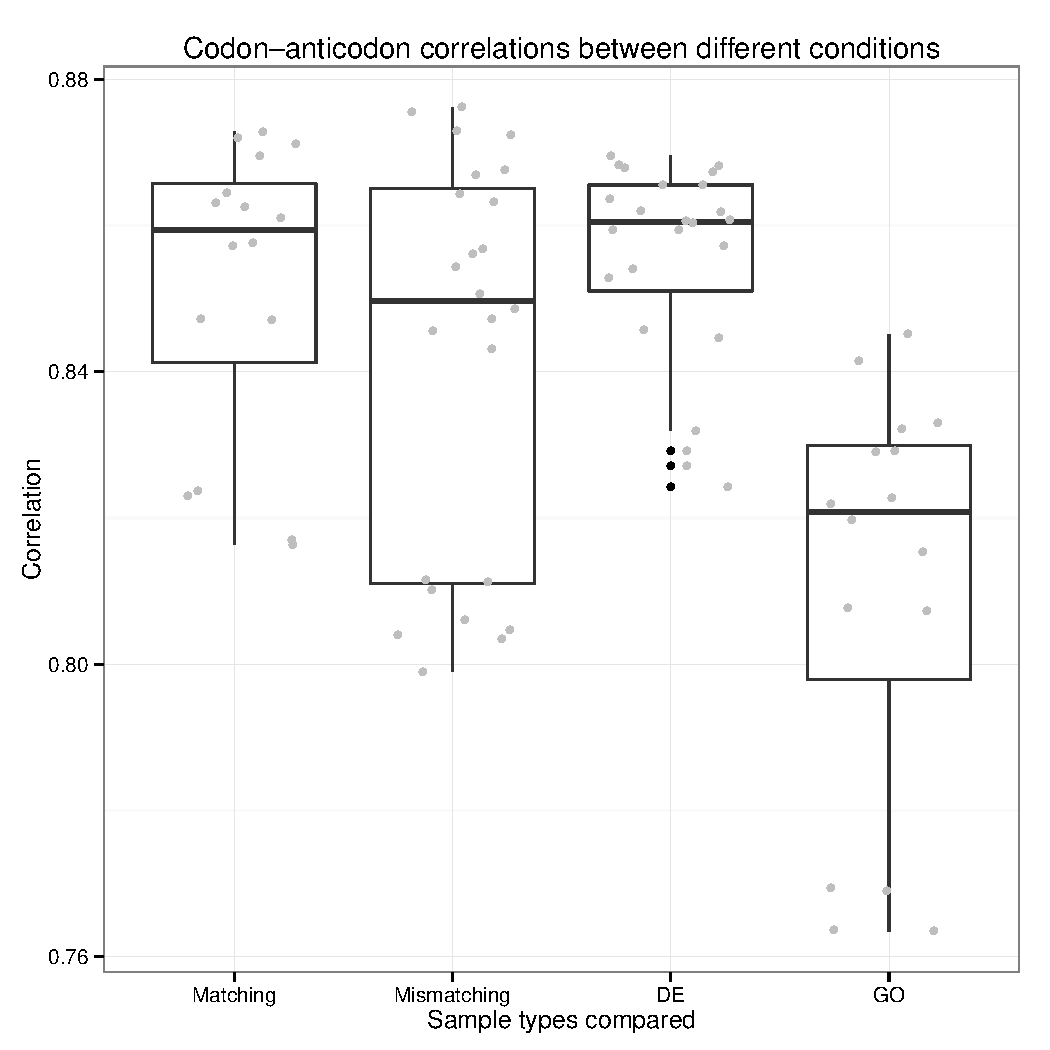
\includegraphics[width=\textwidth]{cub-aab-mouse}%
            \subcaption{\mmu}
        \end{minipage}%
        \begin{minipage}{0.35\textwidth}
            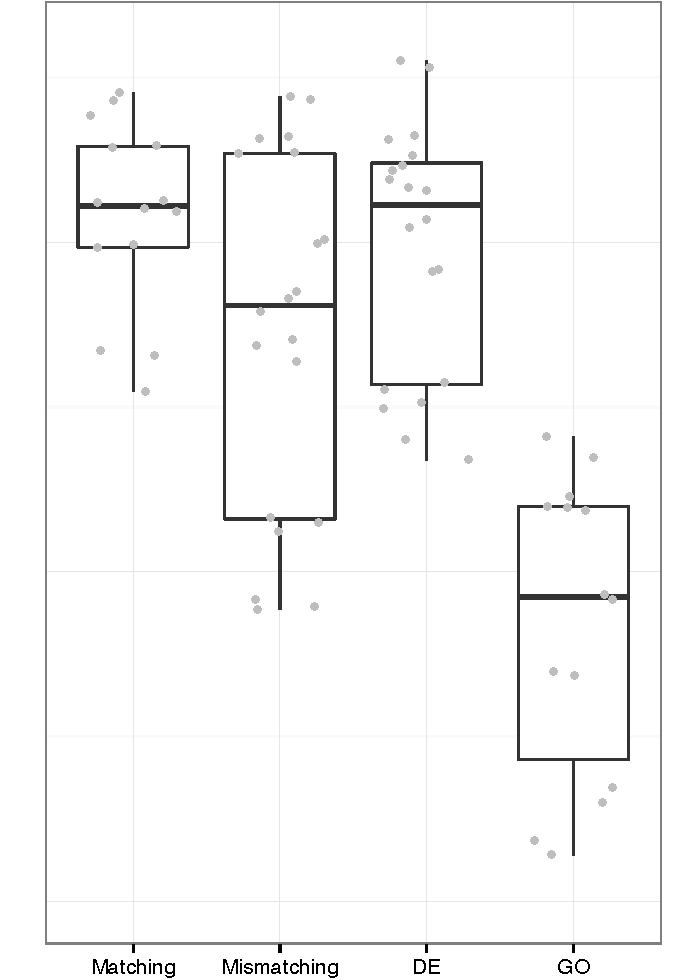
\includegraphics[width=\textwidth]{cub-aab-human}%
            \subcaption{\hsa}
        \end{minipage}%
        \begin{minipage}{0.3\textwidth}
            \scriptsize\sffamily
            \begin{tabu} to \textwidth {@{}ll@{\ --\ }l@{}}
                \toprule
                    & \multicolumn{2}{c}{Contrast} \\
                \midrule
                Matching \\
                \quad\mmu & healthy liver & healthy liver \\
                     & Hepa1-6 & Hepa1-6 \\
                     & Hepa1c1c7 & Hepa1c1c7 \\
                \quad\hsa & healthy liver & healthy liver \\
                     & HepG2 & HepG2 \\
                     & Huh7 & Huh7 \\
                \addlinespace
                Mismatching \\
                \quad\mmu & healthy liver & Hepa1-6 \\
                     & healthy liver & Hepa1c1c7 \\
                \quad\hsa & healthy liver & HepG2 \\
                     & healthy liver & Huh7 \\
                \bottomrule
            \end{tabu}
        \end{minipage}
    }
    {Codon--anticodon correlations.}
    {Each box shows a distribution of codon--anticodon Spearman correlations.
    A codon--anticodon correlation is computed from relative contributions to
    the respective amino acid (i.e.\ \abbr{rcu} versus \abbr{raa}), ignoring
    wobble base pairing. “Matching” shows correlations of the codon and
    anticodon pool of the same condition. “Mismatching” shows correlations of
    the codon and anticodon pool of mismatching conditions (e.g. Hepa1-6 codons
    versus healthy liver anticodons); the two cancer replicates are \emph{not}
    counted as mismatching conditions. “\abbr{de}” shows correlations of the
    codon pool of highly, differentially expressed \mrna genes, and the
    anticodon pool of the same condition. “\abbr{go}” shows correlations of the
    codon pool of condition-specific \abbr{go} term gene sets, and the anticodon
    pool of the same condition. For all distributions, correlations were
    calculated between all pairwise combinations of replicates.}

It is worth nothing that the “\abbr{de}” codon--anticodon correlations vary
non-negligibly, depending on how exactly the top \num{200} condition-specific
genes are chosen; alternative strategies to the one outlined never change the
overall result, however: none of the strategies yielded correlations that were
significantly higher than the transcriptome-wide “matching” correlations.

The current analysis measured \trna anticodon adaptation using the
codon--anticodon correlation, ignoring wobble base pairing. A potentially better
measure of \trna adaptation is the \tai, which accounts for wobble base pairing
in a species-specific manner. Extending the analysis to use the \tai is ongoing
work.

\subsection{Other genomic features may drive the perceived codon usage bias}

The trend seen in \cref{fig:go-cub-pca} does in fact exist to the same degree
when plotting amino acid usage rather than codon usage (\cref{fig:go-aa-pca}).
This suggests that rather than being driven by \go term function, both codon
usage and amino acid usage changes are driven by some other genomic feature. In
fact, the first principal component in \cref{fig:go-cub-pca} correlates almost
perfectly with \gc bias (Pearson’s \(\rho < -0.96\); \cref{fig:cub-vs-gc}).
This has been observed before in other species, for instance in \species{dmel}
and \species{cel} \citep{Duret:2002}. The nature of this relationship is still
unclear and needs to be explored in more detail. In particular, it is unknown
whether \gc bias drives codon bias, or the other way round.

\textfig{go-aa-pca}{body}{0.6\textwidth}
    {\pca of mean \go term amino acid usage.}
    {This figure is analogous to \cref{fig:go-cub-pca}. Each dot corresponds to
    one \go term. The position of the dots is derived by rotating the matrix of
    the mean amino acid usage of the genes belonging to each \go term.}

\textfloat{cub-vs-gc}{spill}
    {%
        \begin{minipage}{0.5\textwidth}
            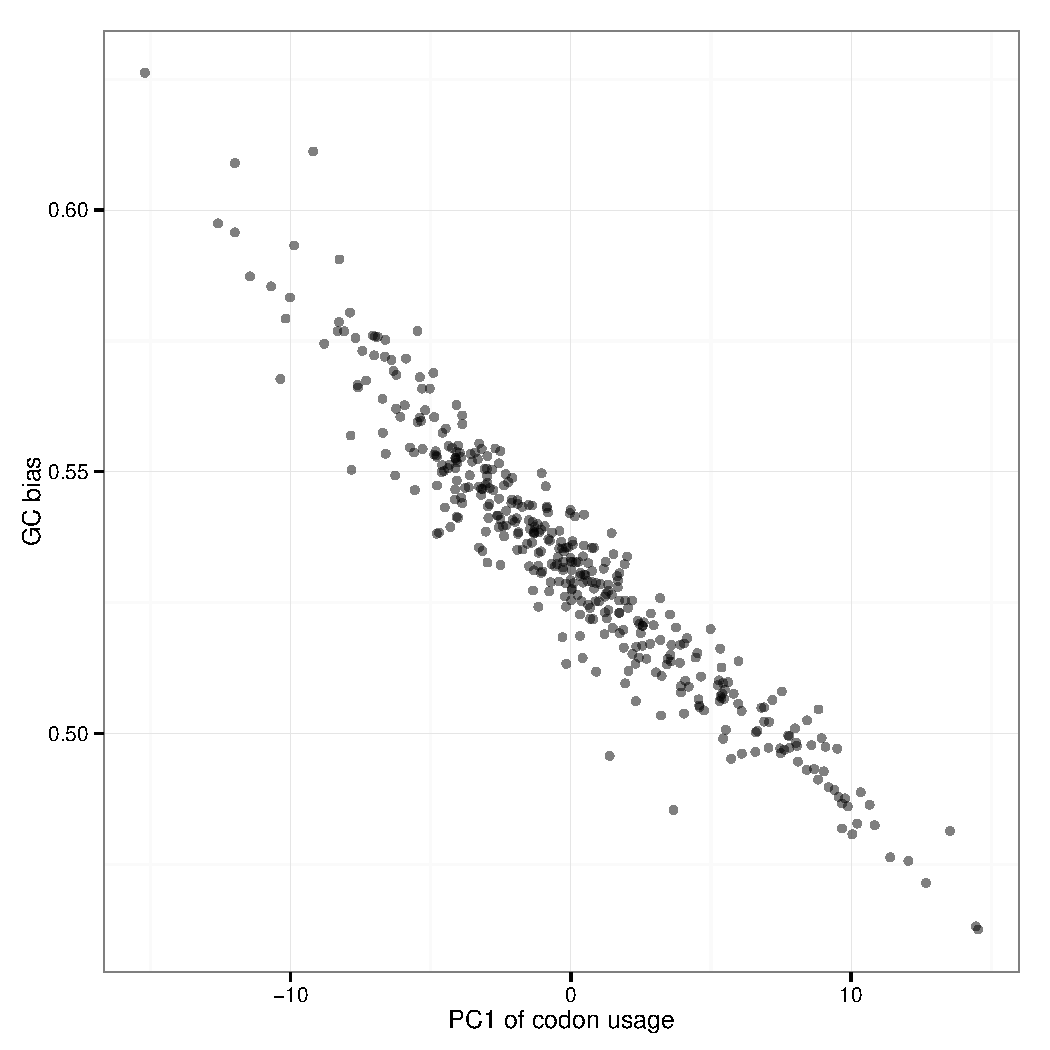
\includegraphics[width=\textwidth]{cub-pc1-vs-gc}%
            \subcaption{\gc bias against codon usage (Pearson’s \(\rho =
            -0.96\)).}
        \end{minipage}%
        \begin{minipage}{0.5\textwidth}
            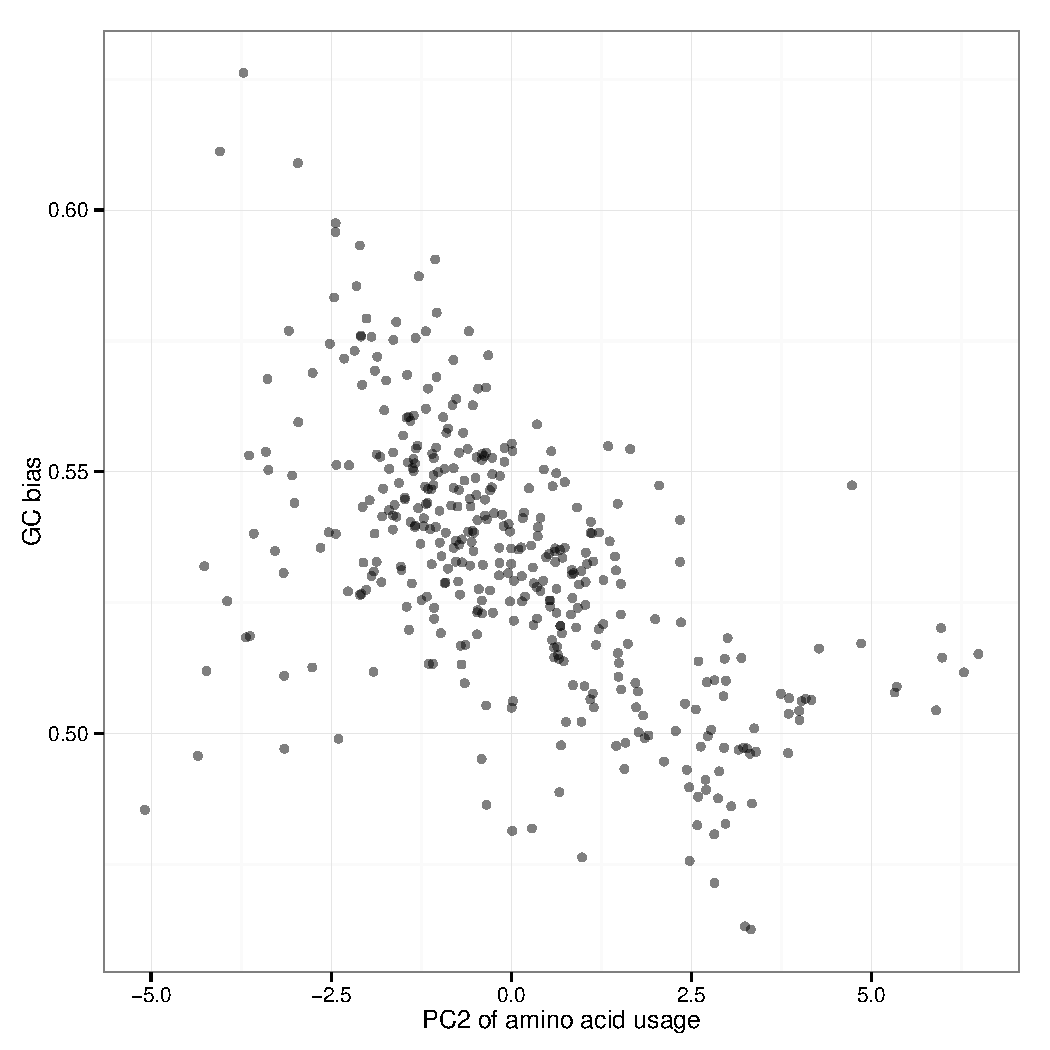
\includegraphics[width=\textwidth]{aa-pc2-vs-gc}%
            \subcaption{\gc bias against amino acid usage (Pearson’s \(\rho =
            -0.58\)).}
        \end{minipage}%
    }
    {\gc bias against a principal component of the \go term codon \& amino acid
    usage \pca.}
    {Each point represents one \go term. The \(x\) coordinate corresponds to
    that of the named principal component of the \pca in
    \cref{fig:go-cub-pca,fig:go-aa-pca}. The \(y\) coordinate corresponds to
    the mean \gc bias of the \go gene set.}

\subsection{Evolutionary conservation of \abbr{trna}--codon adaptation}

If a mechanism leading to the adaptation of the cellular \trna pool to different
cellular conditions existed, we would expect this to be well conserved across
mammalian evolution. Indeed, such an effect should show a \emph{stronger}
conservation of the codon usage bias across different functional gene categories
than conservation of other genomic features, such as the \gc bias. Using genome
data from different mammalian species and homology information for the annotated
\go categories in humans, we can calculate the respective conservation of codon
usage on the one hand, and \gc bias on the other hand. This analysis has not yet
been performed, however.
